\documentclass[11pt]{article}

% Packages
\usepackage{hyperref}
\usepackage{graphicx}
\usepackage{float}

% Margins
\topmargin=-0.45in
\evensidemargin=0in
\oddsidemargin=0in
\textwidth=6.5in
\textheight=9.0in
\headsep=0.25in



\title{Rapport Projet2 - IFT 2015}
\author{ Noms et Matricules : \vspace{0.2cm}\\
	Josué Mongan (20290870) - David Stanescu (20314518)}
\date{Date - 07 juillet 2025}




\begin{document}
	\maketitle	
	\pagebreak
	
	
	\begin{itemize}
		
		\item \underline{Organisation du travail et répartition des tâches}  \vspace{0.2cm}\\
		L'organisation du travail a été assez simple. Premièrement, nous nous sommes donnés du temps individuel pour lire l'énoncé et le comprendre. Une fois cela fait, l'un d'entre nous s'est occupé d'écrire le code pur \texttt{Event} et la \texttt{Simulation} tandis que l'autre s'est occupé de rédiger le code pour la \texttt{Coalescence}. Finalement, nous nous sommes assemblés pour intégrer nos travaux et faire le debugging.
		
		\item \underline{Méthodes de communication et de gestion de code} \vspace{0.2cm}\\
		Pour communiquer, nous avons utilisé comme canal l'application \textbf{Discord} autant par des messages simples que par des appels vocaux avec partage d'écran pour travailler en temps réel sur le code. Pour gérer le code, un \href{https://github.com/Josh012006/Projet2-IFT2015}{répertoire github} a été créé afin d'avoir un meilleur contrôle sur les différentes versions obtenues, les modifications et l'évolution du code.
		
		\item \underline{Explication de l'implémentation} \vspace{0.2cm}\\
		Notre implémentation rajoute au code fourni, les classes \texttt{Event,  Simulation, Coalescence et Main}. 
		\begin{itemize}
			\item La classe \texttt{Event} représente les trois types d'événements avec lesquels notre simulation travaille.
			\item La classe \texttt{Simulation} simule l'évolution de la population dans le temps.
			\item La classe \texttt{Coalescence} est utile pour étudier la coalescence pour les pères et pour les mères.
			\item Dans la classe \texttt{Main}, on récupère les arguments n (la taille de la population intiale) et tMax. On lance ensuite la simulation avant d'étudier la coalescence.
		\end{itemize}
		
		
		\item \underline{Etude empirique des données} \vspace{0.2cm}\\
		Pour notre étude empirique, nous avons lancé la commande
		\texttt{java -jar coalescence-1.0.jar 1000 10000 > sortie.csv} 6 fois et nous avons ensuite étudier la coalescence. Notre étude a porté principalement sur le temps qu'il faut remonter avant de retrouver un ancêtre commun pour toutes la population. \\
		
		Ce que nous avons remarqué est que dans 4/6 des essais, il a suffit de remonter à à peu près la moitié du temps de la simulation pour retrouver des ancêtres communs pour toute la population. Dans les 2/6 des cas, il fallait aller jusqu'au début de la simulation pour les retrouver.\\
		
		\begin{figure}[H]
			\centering
			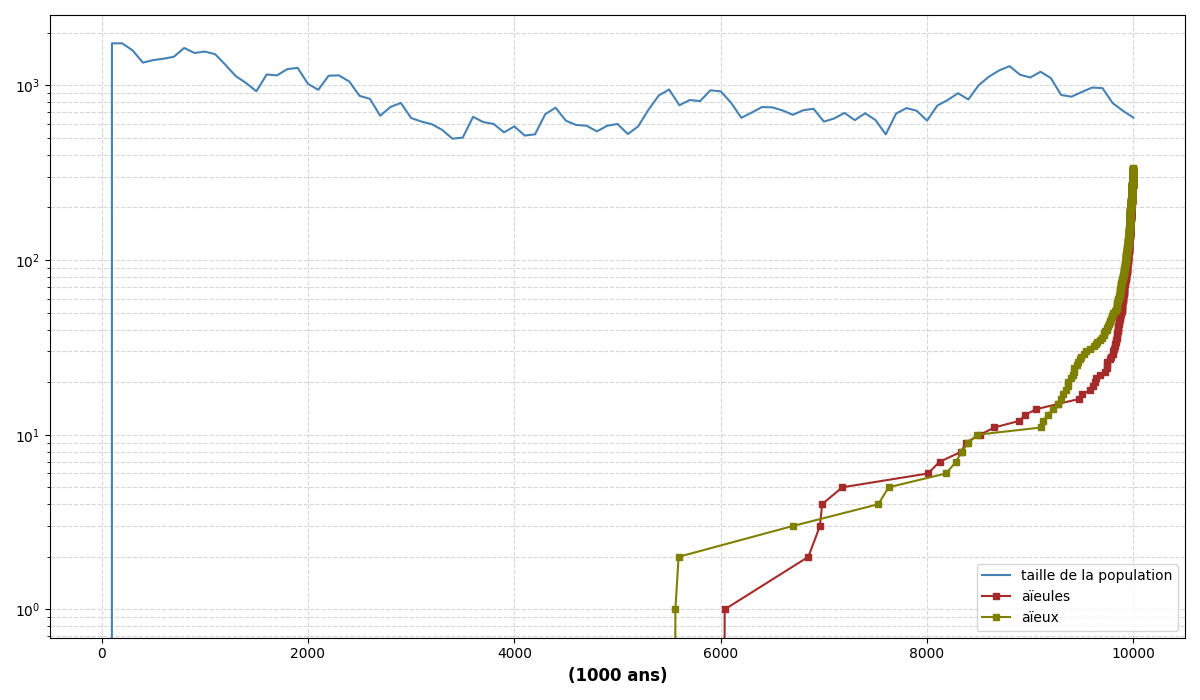
\includegraphics{graphes_population2.png}
			\caption{Aperçu de la coalescence dans 4/6 des cas}
		\end{figure}
		
		\begin{figure}[H]
			\centering
			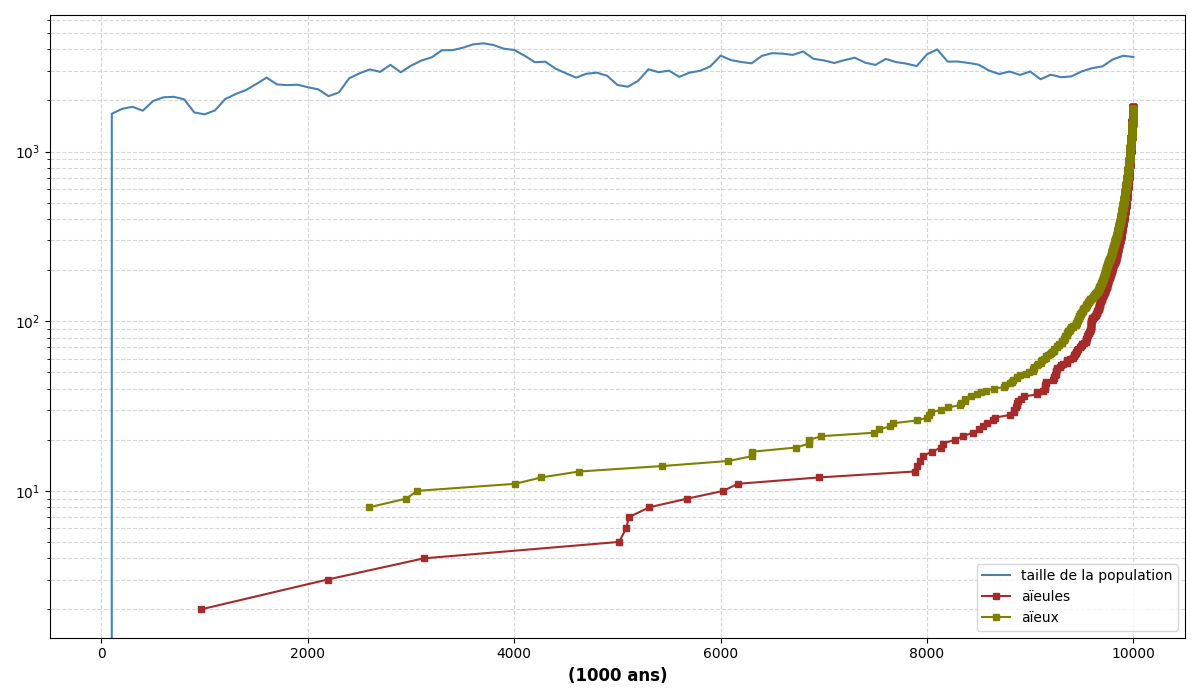
\includegraphics{graphes_population1.png}
			\caption{Aperçu de la coalescence dans 2/6 des cas}
		\end{figure}
		
		La population semble donc avoir été stable pendant un bon moment dans le passé.
		
		
		\item \underline{Utilisation du fichier .jar} \vspace{0.2cm}\\
		Pour utiliser le fichier .jar, il faut écrire dans le terminal, la commande suivante : \texttt{java -jar coalescence-1.0.jar <n> <tMax>}. Par exemple \texttt{java -jar coalescence-1.0.jar 1000 10000}. Le programme affichera sur la sortie standard les valeurs sous format CSV. Premièrement les valeurs liées à la simulation \texttt{Temps,Taille de la population}. Deuxièmement, les valeurs pour la coalescence avec les aïeux \texttt{Temps,Aieux}. Et dernièrement, les valeurs pour la coalescence avec les aïeules \texttt{Temps,Aieules}. \\
		
		Ces valeurs sont affichées les unes à la suite des autres. Il est aussi possible de rediriger cette suite de valeurs dans un fichier CSV par exemple à travers la commande : \texttt{java -jar coalescence-1.0.jar 1000 10000 > sortie.csv}.
		
		
		\item \underline{Difficultés et Bugs} \vspace{0.2cm}\\
		Lors de nos tests, nous avons rencontrés quelques bugs, notamment un premier bug était que notre simulation faisait une boucle infinie. Nous avons facilement repérer le problème qui était au niveau des événements de morts et de la mise à jour du temps courant. Le deuxième bug qui a été un peu plus complexe à régler était que nous avions des données non représentative pour la coalescence. Les graphes générés ne ressemblaient pas à une étude coalescence sur une population. Mais le bug était au niveau du \texttt{Comparator} passé à la \texttt{PriorityQueue}. Une fois réglé, notre code était complètement fonctionnel et satisfaisant.
		
		\item \underline{Temps passé sur le travail} \vspace{0.2cm}\\
		Le temps total passé sur le travail par l'équipe (lecture + compréhension + écriture du code + débogage) est d'environ \textbf{15 heures}.
		
	\end{itemize}	
	
	
	
\end{document}